\documentclass[11pt]{article}
\usepackage[margin=1in]{geometry}
\usepackage[T1]{fontenc}
\usepackage[utf8]{inputenc}
\usepackage{lmodern,microtype}
\usepackage{amsmath,amssymb,amsthm,mathtools}
\usepackage{graphicx,booktabs,array,enumitem,setspace,placeins}
\usepackage{algorithm}
\usepackage{algpseudocode}
\usepackage{needspace}
\usepackage[authoryear,round]{natbib}
\usepackage[colorlinks=true,allcolors=blue]{hyperref}
\usepackage{bookmark}
\allowdisplaybreaks
\setstretch{1.18}
\setlength{\parskip}{0pt}
\setlength{\emergencystretch}{2em}
\setlist{itemsep=2pt,topsep=4pt}
\newtheorem{theorem}{Theorem}[section]
\newtheorem{lemma}[theorem]{Lemma}
\newtheorem{proposition}[theorem]{Proposition}
\newtheorem{corollary}[theorem]{Corollary}
\newtheorem{definition}[theorem]{Definition}
\newtheorem{example}[theorem]{Example}
\theoremstyle{remark}
\newtheorem{remark}[theorem]{Remark}
\newcommand{\E}{\mathbb E}
\newcommand{\Prob}{\mathbb P}
\newcommand{\ind}{\mathbf 1}
\newcommand{\kl}{\operatorname{kl}}
\newcommand{\pos}[1]{\left[#1\right]_+}
\newcommand{\suppproof}{Complete proofs appear in the supplementary material.}

% Set \anonymoustrue for an author-free review copy if required by the portal.
\newif\ifanonymous
\anonymousfalse
\title{Multi-armed bandits with arriving arms:\\
sequential screening and reliable set maintenance}
\ifanonymous
\author{}
\else
\author{Deqi Zheng\thanks{The first two authors contributed equally.} \quad
 Xiaoyang Xu\footnotemark[1] \\ Qiuzhen College, Tsinghua University
 \and Yuhong Yang\thanks{Corresponding author: yyangsc@mail.tsinghua.edu.cn.}\\
 Yau Mathematical Sciences Center, Tsinghua University}
\fi
\date{October 15, 2026}
\begin{document}
\maketitle

\begin{abstract}
We study a stochastic multi-armed bandit problem in which new arms arrive
exogenously and remain available. Performance is measured against the best
currently available arm. The resulting arrival information discrepancy and
drifting benchmark motivate UCB for Arriving Arms (UCB-AA), which screens new
arms before they enter full competition with incumbents. We analyze this
two-stage design and give a finite-budget regret analysis based on the
comparisons and sample prefixes actually used. The analysis separates learning
among admitted arms from delayed admission and loss of an earlier benchmark.
We then ask what statistical benefit can accompany screening beyond a smaller
internal active set. For simultaneous, reliable reporting of the relative
near-optimal set, uncertainty about one arrival can obstruct many earlier
certifications. We characterize a worst-schedule maintenance cost and identify
the polynomial arrival boundary for sublinear unresolved time. A repeated-update
family shows that prompt resolution of temporary membership questions can
require inverse-square regret, whereas allowing more waiting admits a
logarithmic upper bound. The necessary cost also holds with fixed positive
probability. A separate checkpoint construction supplies attainable reporting
bounds. Numerical evidence distinguishes the archived UCB-AA implementation
from this construction and exposes the finite-budget cost of conservative
certification.
\end{abstract}
\noindent\textit{Keywords:} sequential experimentation; adaptive screening;
arriving arms; dynamic regret; arrival information discrepancy; drifting benchmark.

\section{Introduction}
\label{sec:introduction}

The classical multi-armed bandit framework assumes that the set of available actions is fixed in advance. In many modern applications, however, the action set expands over time. Precision oncology provides a representative example: as genomic profiling has advanced, the set of approved targeted therapies for non-small cell lung cancer has grown substantially, so a trial designed around a fixed collection of treatments may become outdated before it is completed. Similar issues arise in online advertising and other adaptive decision problems in which new options appear sequentially.

\begin{figure}[t]
\centering
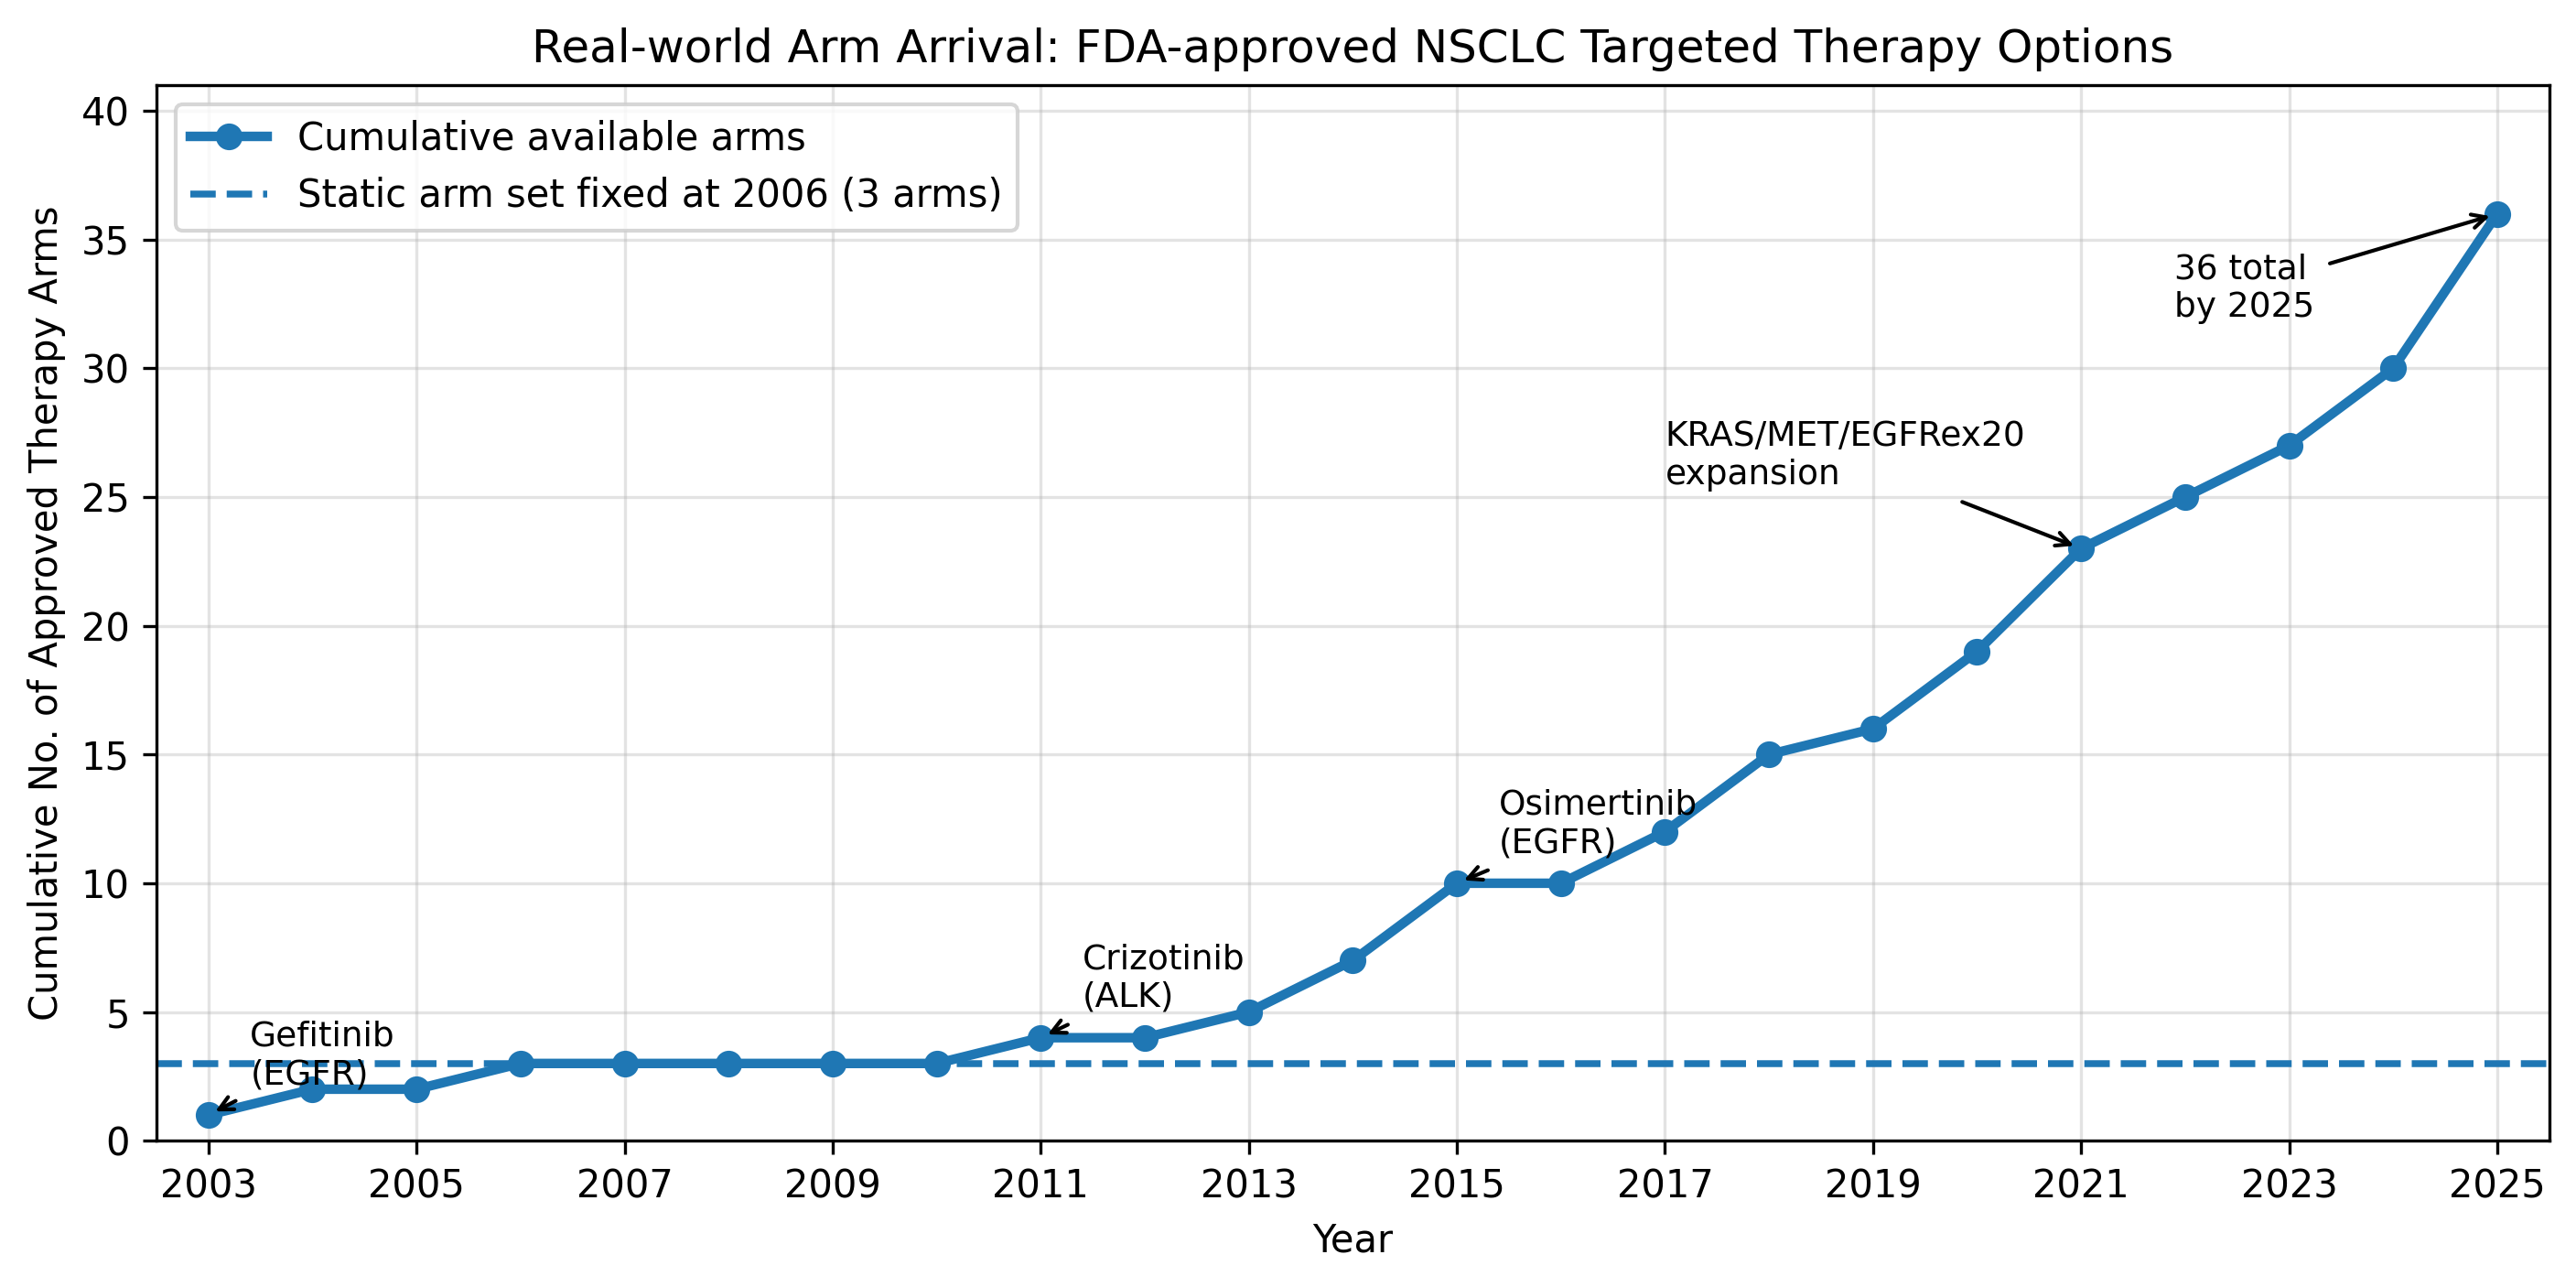
\includegraphics[width=.76\textwidth]{figures/original_submission/figure_nsclc_targeted_therapy_arms.png}
\caption{The historical motivating illustration from the original submission:
FDA approval records for targeted therapies and immunotherapies for
non-small cell lung cancer over 2003--2025 \citep{FDA_DrugsFDA}.
The expanding option set motivates arriving-arm experiments. No treatment
outcomes from this illustration enter the bandit simulations.}
\label{fig:nsclc_growth}
\end{figure}

Motivated by such problems, we study the \emph{multi-armed bandit problem with
arriving arms} (MAB-AA). Let $\mathcal A_t$ denote the set of arms available at
time $t$, with $\mathcal A_t\subseteq\mathcal A_{t+1}$. New arms arrive over time
and remain available thereafter. Performance is evaluated against the best arm
currently available, since a terminal best arm need not have been available
earlier.

Relative to the classical stochastic bandit setting, MAB-AA introduces two main difficulties. The first is \emph{arrival information discrepancy (AID)}: newly arrived arms must be explored, which repeatedly diverts samples away from well-understood incumbent arms. The second is a \emph{drifting benchmark (DB)}: as better arms enter the system, both the identity of the optimal arm and the regret benchmark may change over time.

The setting retains stationary, unstructured reward laws and an external
arrival process. Arms are not drawn on demand from a reservoir
\citep{10.1214/aos/1069362389}, and do not disappear as in mortal bandits
\citep{NIPS2008_788d9869}. Permanent arrivals are a monotone special case of
sleeping-bandit availability \citep{kleinberg2010}. Benchmark changes are caused
by new arms, rather than changes in the reward laws of existing arms as in
nonstationary bandits \citep{Besbes2014,Auer2019ADSWITCH}.
Ballooning bandits already use permanent arrivals and regret against the best
currently available arm \citep{ghalme2021}; we do not claim either as a new model
or comparator.

From a statistical perspective, multi-armed bandit problems have long been studied as models for sequential allocation and adaptive experimentation, dating back to \citet{Robbins1952} and the asymptotically efficient allocation theory of \citet{LAI19854}; see also \citet{Lai1987} for connections to adaptive treatment allocation. This viewpoint has motivated a broad statistical literature, including Bayesian and index-based approaches to sequential allocation \citep{Gittins1979,BerryFristedt1985}, response-adaptive randomization in clinical trials \citep{Zelen1969,WeiDurham1978,VillarBowdenWason2015,WilliamsonVillar2020,AzizKaufmannRiviere2021}, covariate-dependent and nonparametric bandit methods \citep{Woodroofe1979,YangZhu2002,RigolletZeevi2010,PerchetRigollet2013}, and recent high-dimensional, semiparametric, and transfer-learning formulations \citep{QianYang2016,QianIngLiu2023,CaiCaiLi2024}. These works share with ours the broad goal of learning from accumulated evidence to reduce allocation to inferior alternatives, but do not directly study the permanent exogenous arrival setting considered here.

Methodologically, the two challenges call for different but complementary design principles. To address AID, our approach combines elimination steps \citep{EvenDar2006SE,Auer2010UCBRI,PerchetRigollet2013,QianYang2016} with a pre-elimination mechanism tailored to the expanding action set. The key idea is to prevent the main competition stage from being repeatedly disrupted by every newly arriving arm. Instead, late arrivals are first screened against incumbent candidates, so that clearly inferior arms can be removed before receiving the full exploration budget assigned to serious contenders. To handle DB, the algorithm repeatedly updates the relevant comparison set as new arms arrive, and the analysis evaluates regret against the best arm currently available rather than against a fixed hindsight oracle. 
% This leads to a regret decomposition that separates the cost of certifying new arrivals from the delay cost incurred before the learner catches up with a newly improved benchmark.
Based on these ideas, we propose \textbf{UCB for Arriving Arms (UCB-AA)}. For UCB-AA, we derive regret upper bounds that depend explicitly on the arrival process, establish sublinear dynamic regret when arm-count growth and admission delay are controlled, study representative lower-bound regimes, and develop an online extension for unknown horizons.

UCB for Arriving Arms (UCB-AA) implements this screening design. Its
pre-elimination stage samples an arrival at coarse resolutions before spending
the finer budget used for incumbent arms. Formal elimination then compares the
merged active set. A finite-budget analysis must account for unfinished phases,
arrivals waiting for admission, and any loss of a previously admitted best arm.
We give that accounting explicitly and establish a sample-count bound without
compressing historical gaps into a terminal gap.

The active set alone does not describe what has been learned about all
available arms. An excluded arm may be statistically inferior, or it may never
have been admitted. This distinction leads to a further question within the
same MAB-AA setting: what does it cost to maintain reliable knowledge of the
complete relative near-optimal set while collecting reward? The fixed-arm
version is the ALL-$\varepsilon$ problem \citep{mason2020}. Joint reward and
identification objectives also have established precedents
\citep{degenne2019,yang2026,cho2025}. Our additional requirement concerns
continuing reports under arrivals, with one simultaneous correctness event and
a cumulative cost for unresolved arm time.

Two effects of the drifting benchmark determine that cost. An uncertain new
arm can block positive certification of many well-studied incumbents. A later
improvement can also make a difficult earlier membership question irrelevant.
We prove a common-environment broadcast lower bound and a worst-schedule
maintenance bound, obtaining the polynomial arrival exponent below which
sublinear regret and sublinear unresolved time are jointly possible. In a
repeated-update family, prompt maintenance has matching inverse-square regret
bounds at specified horizons, whereas a larger constant-factor area budget
admits a logarithmic regret upper bound. A fixed-probability lower bound shows
that the necessary cost is not confined to rare paths. These are substantive
extensions of the original regret question, rather than guarantees inferred
from the size of UCB-AA's active set.

For the reporting upper bounds we use a separate checkpoint construction,
CP-UCB-AA. It preserves accumulated observations but does not remove negatively
reported arms from reward selection. We distinguish its guarantees from those
of the two-stage UCB-AA procedure. The numerical study likewise distinguishes
the original archived implementation from the reporting comparisons. It
retains favorable and unfavorable original observations, while showing that
conservative fixed checkpoints can be impractical at moderate budgets.

\section{Multi-armed bandit problem with arriving arms}
\label{sec:model}
\label{sec:problem}
\subsection{Problem formulation}

We consider a sequential decision process over time steps $t=1,2,\ldots$.
Let $\mathcal A$ be the possibly infinite set of all arms. At time $t$ only
$\mathcal A_t\subseteq\mathcal A$ is available, where
$\mathcal A_t\subseteq\mathcal A_{t+1}$,
$\mathcal A_1\ne\varnothing$, and $K_t=|\mathcal A_t|<\infty$.
For arm $i$, its arrival time is
\[
 \tau_i=\inf\{t\ge1:i\in\mathcal A_t\}.
\]
Each arm has an unknown stationary reward law on $[0,1]$ with mean $r_i$.
Reward streams are independent across arms, and successive observations of
each arm are independent and identically distributed. The arrival process is
exogenous to the learner and independent of these reward streams. We state
results conditional on a fixed arrival schedule unless otherwise specified.

In physical-time notation, $X_{t,i}$ denotes the reward observed if arm
$i$ is selected at time $t$. A policy is a sequence
$\pi=(\pi_t)_{t\ge1}$ of possibly randomized rules. After seeing
$\mathcal A_t$, it selects $I_t\in\mathcal A_t$ using the observed history
\[
 H_{t-1}=(\mathcal A_s,I_s,X_{s,I_s})_{s=1}^{t-1}
\]
and independent randomization, and then observes $X_{t,I_t}$.
It does not know the arm means or future arrivals.

Write $N_i(t)=\sum_{s\le t}\ind\{I_s=i\}$ for the cumulative number of pulls
of arm $i$. To distinguish pull number from physical time, represent its
successive potential observations by $(Y_{i,n})_{n\ge1}$, so that
$X_{t,I_t}=Y_{I_t,N_{I_t}(t-1)+1}$. Define
\[
 \hat r_i(n)=\frac1n\sum_{s=1}^nY_{i,s},\qquad
 r^*(t)=\max_{i\in\mathcal A_t}r_i,\qquad
 \Delta_i(t)=r^*(t)-r_i\quad(i\in\mathcal A_t).
\]
For an almost surely finite stopping time $\tau$, the cumulative dynamic regret is
\[
 R_\tau(\pi)=\sum_{t=1}^{\tau}\bigl(r^*(t)-r_{I_t}\bigr).
\]
At a deterministic horizon $T$ we write $R_T(\pi)$, or $R_T$ when the policy
is understood. It is random through the arm selections; $\E R_T$ is its
expectation. A definition at random $\tau$ does not assert that every
deterministic-horizon bound also holds at arbitrary stopping times.
Physical time $t$ always counts actual pulls. Algorithmic rounds are indexed
separately by $m$.

\subsection{Main statistical challenges}

\textbf{Arrival information discrepancy (AID).}
A first difficulty is arrival information discrepancy. With a finite sampling budget up to time $T$, the learner must allocate samples both to incumbent arms and to newly arriving arms whose rewards are still highly uncertain. Under continual arrivals, this repeated re-exploration can prevent the learner from concentrating pulls on the best currently available arm. Consequently, without additional regularity conditions on the arrival process, sublinear regret may be unattainable.

\textbf{Drifting benchmark (DB).}
In contrast to the classical setting where the best mean reward is fixed, the benchmark in MAB-AA is time-dependent: $r^*(t)=\max_{i\in \mathcal{A}_t} r_i$. Since $\mathcal{A}_t$ expands over time, both the identity of the best arm and the value $r^*(t)$ may change when new arms arrive. Consequently, for a fixed arm $i$, the suboptimal gap $r^*(t)-r_i$ is generally time-varying (and non-decreasing in $t$). This drifting benchmark complicates both algorithm design and analysis, because the learner must continuously compare well-sampled incumbent arms with newly arriving arms whose estimates are still highly uncertain.

\subsection{Admission and retirement in the reward account}

The distinction between statistical reports and reward eligibility is useful
even before introducing a policy. Let $\mathcal{A}^{\mathrm{adm}}_t\subseteq \mathcal{A}_t$ be an admitted set and
$B_t\subseteq \mathcal{A}^{\mathrm{adm}}_t$ its nonempty reward-active subset, with $I_t\in B_t$.
At every deterministic endpoint, including one inside an algorithmic round,
\begin{align}
 R_T={}&\sum_{t\le T}(\max_{i\in B_t}r_i-r_{I_t})
 +\sum_{t\le T}(r^*(t)-\max_{i\in \mathcal{A}^{\mathrm{adm}}_t}r_i)\notag\\
 &+\sum_{t\le T}(\max_{i\in \mathcal{A}^{\mathrm{adm}}_t}r_i-\max_{i\in B_t}r_i).
 \label{eq:three_part}
\end{align}
This follows by adding and subtracting the two intermediate maxima at each
pull. The terms are within-active learning, admission delay, and loss of an
admitted benchmark through retirement. The latter two cannot in general be
identified with arrival increments alone. On a simultaneous confidence event, the revised UCB-AA comparisons preserve
a best admitted arm, making the third term zero. The checkpoint construction
introduced later uses $B_t=\mathcal{A}^{\mathrm{adm}}_t=\mathcal{A}_t$
for reward selection, so its last two terms vanish on every sample path.


\section{UCB for Arriving Arms (UCB-AA)}
\label{sec:algorithm}

UCB-AA is an elimination-based procedure organized by rounds. Its main idea is simple:
newly arriving arms are not allowed to compete immediately with well-sampled incumbent
arms. Instead, they are first buffered and screened at lower cost. Only those that survive
this screening step enter full competition in the next stage. This design aims to reduce
wasted exploration on clearly suboptimal late arrivals while preserving the ability to detect
genuinely competitive new arms.

% Proposed replacement block for the original UCB-AA analysis.
% Root agent will inline this into the single-file main manuscript.
% Complete proofs: theory/ucbaa_repaired_analysis.tex.
\subsection{UCB-AA under a physical sampling budget}
\label{sec:ucbaa_fixed_budget}

UCB for Arriving Arms (UCB-AA) uses two stages of screening.
At the beginning of round $m$, admit the buffered batch $A_m$ and form
$B_m=C_{m-1}\cup A_m$, where $C_{m-1}$ contains the surviving incumbents.
For $m\ge2$, screen the new arms in phases $p=0,\ldots,m-2$ against
the incumbents and the remaining new arms; only new arms can be removed.
Then apply formal elimination to the merged set in phases $m-1,m$.
Round zero uses phase zero, and round one uses formal phases zero and one.
Empty preliminary batches are no-ops. This retains the distinction between
pre-elimination, which addresses arrival information discrepancy, and
formal elimination after new arms have entered the main competition.

Let $s_m$ be the physical start of round $m$. Set $A_0=\mathcal A_1$ and,
for $m\ge1$, admit the entire buffer, including arrivals at $s_m$:
$A_m=\mathcal A_{s_m}\setminus A(m-1)$, where
$A(m-1)=\bigcup_{j<m}A_j$. Arrivals during a call are added to the
buffer before the current physical action and wait for the next round.

To give this procedure a fixed-budget guarantee, specify its confidence
calibration, comparison data, and stopping rule. For a known physical
budget $T\ge1$ and $0<\delta<1$, let
\begin{equation}
 M_T=\left\lceil\tfrac12\log_2(T+1)\right\rceil,\qquad
 N=8T4^{M_T}/\delta,\qquad\widetilde\Delta_p=2^{-p}.
 \label{eq:ucbaa_main_calibration}
\end{equation}
Use the target and radius formulas
\begin{equation}
 n_p=\left\lceil
       \frac{2\log(N\widetilde\Delta_p^2)}{\widetilde\Delta_p^2}
      \right\rceil,\qquad
 b_p=\sqrt{\frac{\log(N\widetilde\Delta_p^2)}{2n_p}}.
 \label{eq:ucbaa_main_targets}
\end{equation}
In an elimination call, sample each candidate to $n_p$ lifetime pulls,
retaining all earlier observations. After the call's sampling is complete,
compare the actual prefix intervals
$\hat r_i(n_p)\pm b_p$. Remove a candidate only if its upper bound is
strictly below the largest reference lower bound. Incumbents have already
reached the necessary prefix before a preliminary comparison, so no
unobserved incumbent estimate is used. Stop after physical pull $T$,
including when it cuts through a target or a round. The calibrated
$n_{M_T}>T$ ensures that the finite phase range covers this execution.
These conventions specify the confidence comparisons and budget accounting
for the two elimination stages. The guarantee below uses this calibration; a smaller empirical
calibration need not have the same coverage probability.


\begin{algorithm}[t]
\caption{UCB for Arriving Arms (UCB-AA), with explicit prefix comparisons}
\label{alg:ucb-aa}
\small
\begin{algorithmic}[1]
\Require Physical budget $T$; $M_T,N,n_p,b_p$ from
\eqref{eq:ucbaa_main_calibration}--\eqref{eq:ucbaa_main_targets}
\State Initialize $C_{-1}=\varnothing$ and retain lifetime sample prefixes
\State Stop immediately after pull $T$; an unfinished call performs no elimination
\Procedure{Elim}{$S,R,p$}
    \State Before each physical pull, add newly arriving unadmitted arms to the buffer
    \State Pull each $j\in S$ to $n_p$ total observations
    \State For $j\in R$, set $\mathrm{LCB}_j=\hat r_j(n_p)-b_p$,
           $\mathrm{UCB}_j=\hat r_j(n_p)+b_p$
    \State Remove simultaneously from $S$ every $j$ with
           $\mathrm{UCB}_j<\max_{i\in R}\mathrm{LCB}_i$
    \State \Return $S$
\EndProcedure
\For{$m=0,\ldots,M_T$}
    \State Admit buffered batch $A_m$; set $B_m^0=C_{m-1}\cup A_m$
    \If{$m\ge2$}
        \State Set $A_m^0=A_m$
        \For{$p=0,\ldots,m-2$}
            \If{$A_m^p\ne\varnothing$}
                \State $A_m^{p+1}\gets\Call{Elim}{A_m^p,C_{m-1}\cup A_m^p,p}$
            \Else
                \State $A_m^{p+1}\gets\varnothing$
            \EndIf
            \State $B_m^{p+1}\gets C_{m-1}\cup A_m^{p+1}$
        \EndFor
    \EndIf
    \If{$m=0$}
        \State $B_m^1\gets\Call{Elim}{B_m^0,B_m^0,0}$
    \Else
        \For{$p=m-1,m$}
            \State $B_m^{p+1}\gets\Call{Elim}{B_m^p,B_m^p,p}$
        \EndFor
    \EndIf
    \State $C_m\gets B_m^{m+1}$
\EndFor
\end{algorithmic}
\end{algorithm}

The algorithm retains the original two stages. Pre-elimination applies only
to newly admitted arms and uses the already observed incumbent prefixes.
Formal elimination applies to the merged active set. The empty-batch branch,
strict comparison, and physical-budget stopping rule make those operations
unambiguous; they do not replace screening with the checkpoint construction.

\subsection{Roundwise regret, historical loss, and arrival delay}
\label{sec:ucbaa_three_contributions}

Let $s_m$ be the physical start of round $m$,
$A(m)=\bigcup_{j\le m}A_j$, and
$r_{*(m)}=\max_{i\in B_m}r_i$.
Write $\Delta_i^{\mathrm{rd}}(m)=r_{*(m)}-r_i$ for its roundwise gap,
reserving $\Delta_i(t)=r^*(t)-r_i$ for physical time.
Write $r_{\mathrm{adm}}(m)=\max_{i\in A(m)}r_i$ for the best mean
among all admitted arms, including those previously eliminated.
At a physical time $t$, the current round is $m(t)$. The exact regret
identity is
\begin{align}
 R_T(\pi)&=R_{\mathrm{round}}(T)+\mathcal H_T+D_T,\label{eq:ucbaa_main_decomposition}\\
 R_{\mathrm{round}}(T)
  &=\sum_{t\le T}\{r_{*(m(t))}-r_{I_t}\},\nonumber\\
 \mathcal H_T&=\sum_{t\le T}\{r_{\mathrm{adm}}(m(t))-r_{*(m(t))}\},\nonumber\\
 D_T&=\sum_{t\le T}\{r^*(t)-r_{\mathrm{adm}}(m(t))\}.\nonumber
\end{align}
All three quantities are nonnegative. The historical term $\mathcal H_T$ records
the consequence of eliminating an admitted benchmark arm; $D_T$ records
only the time before arrivals are admitted. Combining them into a residual
does not make that residual arrival delay.

For a complete run of $M+1$ rounds, the original $T_0(\pi)$ denotes its
actual random number of pulls, and
$R_{\mathrm{round}}(T_0(\pi))=R_M(\pi)$.
The pathwise identity also applies at this endpoint, but the fixed-budget
bound does not replace $T$ by $\mathbb E T_0(\pi)$ or assert a guarantee
for an arbitrary stopping time. The original $K(m)$, if supplied, bounds
$|A(m)|$; it differs from the actual count $K_t=|\mathcal A_t|$ and is
not an additional input required by the present calibration.

The delay contribution is explicit. Let
$\beta_u=r^*(u)-r^*(u-1)$ for $u\ge2$ and let $\alpha_T(u)$ be the
first round start at or after $u$, with value $T+1$ when no such start
occurs by $T$. Because $A(m)=\mathcal A_{s_m}$,
\begin{equation}
 D_T=\sum_{u=2}^T\beta_u\{\alpha_T(u)-u\}.
 \label{eq:ucbaa_main_delay}
\end{equation}
This formula retains benchmark improvements in the last unfinished round.

\begin{theorem}[A repaired fixed-budget bound for UCB-AA]
\label{thm:ucbaa_main_fixed_budget}
For independent arm streams, each consisting of iid $[0,1]$-valued rewards,
deterministic permanent arrivals, a nonempty initial arm set, and
$K_T=|\mathcal A_T|<\infty$,
the UCB-AA procedure specified
above satisfies, with probability at least $1-\delta$,
\[
 \mathcal H_T=0,\qquad
 R_T(\pi)\le\min\{T,\ 8\sqrt{(2\log N+1)K_TT}+D_T\}.
\]
It follows that
\begin{equation}
 \mathbb E R_T(\pi)\le
 \min\{T,\ 8\sqrt{(2\log N+1)K_TT}
                  +\mathbb E D_T+\delta T\}.
 \label{eq:ucbaa_main_bound}
\end{equation}
The inequalities include incomplete targets and rounds and allow ties
between arm means. No terminal-gap stability condition is needed.
\end{theorem}

The proof uses the actual lifetime observation count. On one simultaneous
prefix-coverage event, a best admitted arm survives every comparison.
A new arm that receives phase-$p$ samples for $p\ge1$ has survived the
preceding comparison in the same round; its roundwise gap is at most
$4b_{p-1}$. An incumbent receives no new samples in formal phase $m-1$,
because it already has $n_{m-1}$ observations. Its new phase-$m$ samples
follow the current round's phase-$m-1$ comparison and obey the same bound.
Thus the $n$th observation of an arm has roundwise loss at most
$4\sqrt{(2\log N+1)/n}$. Summing these distinct prefix charges yields
\eqref{eq:ucbaa_main_bound}; the argument does not replace intermediate gaps by a terminal gap
or condition on a selected elimination chain. The supplementary material
gives the full proofs.

For $T\ge2$, the choice $\delta=T^{-2}$ makes the statistical term
$O(\sqrt{K_TT\log(T+1)})$. Sublinear regret therefore follows under
the sufficient conditions $K_T\log(T+1)=o(T)$ and
$\mathbb E D_T=o(T)$. The delay condition is essential to this statement;
the result does not assert sublinear regret for arbitrary arrivals.
For an unknown horizon, a restart at physical budgets $1,2,4,\ldots$
gives a valid extension with the same statistical order and its own explicit
delay term. The supplementary material provides its construction.
Each restart has a prescribed number of physical pulls, so an
unfinished round is charged at the actual endpoint.

\begin{corollary}[Static arms and fixed-gap distractors]
\label{cor:ucbaa_main_fixed_gap}
Suppose an arm available at time one has mean $r^\star$ and every arm
arriving by $T$ has mean at most $r^\star$. Write
$\Delta_i=r^\star-r_i$ and $A=2\log N+1$. Then $D_T=0$ pathwise and,
with probability at least $1-\delta$,
\begin{equation}
 R_T(\pi)\le\sum_{\substack{i\in\mathcal A_T\\\Delta_i>0}}
       \min\left\{\Delta_i(T-\tau_i+1),\frac{16A}{\Delta_i}\right\}.
 \label{eq:ucbaa_main_fixed_gap}
\end{equation}
Adding $\delta T$ gives an expected-regret bound, and both bounds may
be capped at $T$.
\end{corollary}

Indeed the active best mean equals $r^\star$ on the common confidence
event. Applying the actual-prefix charge to a suboptimal arm's last
observation gives $N_i(T)\le16A/\Delta_i^2$, while
$N_i(T)\le T-\tau_i+1$. For $T\ge2$ and $\delta=T^{-2}$, the static case therefore
has upper order $\sum_{i:\Delta_i>0}\log(T+1)/\Delta_i$; arrivals with
a fixed positive gap have upper order $K_T\log(T+1)$.
For example, consider an initial optimum
$r^\star=3/4$, another initial mean $1/4$, and arriving means
$r_i=1/2-2^{-i-2}$ at exogenous physical times $\tau_i$, $i\ge1$.
All distractors have gap at least $1/4$, so the same bound gives
$O(K_T\log(T+1))$ expected regret for this exogenous arrival example.

% Retained original regret lower bounds, for insertion into the main source.
% Original source: mab_aa_main.tex lines 1002--1179 and 1215--1355.
% The local-alternative proof is replaced; no original UCB-AA upper claim is used.
\section{Regret lower bounds in representative arrival regimes}
\label{sec:retained_regret_lower_bounds}

We consider two representative lower-bound regimes for regret.
The first describes the evidence needed to reject inferior arrivals when
the best arm is already available. Its static special case is a classical
calibration \citep{LAI19854,BurnetasKatehakis1996}. The second describes
successive local comparisons as the benchmark improves. Both concern regret
at a deterministic physical horizon. They are separate from the reporting
requirements introduced below, and are not claimed as matching converses to
an upper bound evaluated at a random round-completion time.

\subsection{Static arms and arriving distractors}

For each horizon $T$, fix an exogenous deterministic arrival schedule and a
baseline environment $\nu^{(0)}$. Arm $0$ is available from time $1$ and has
mean $r^\star$ strictly larger than every other mean. Let $\mathcal I_T$ be
a nonempty collection of inferior arrivals. For $i\in\mathcal I_T$, write
\[
 r_i=r^\star-\Delta_i,\qquad
 H_i(T)=T-\tau_i+1,\qquad
 H_{\min}(T)=\min_{i\in\mathcal I_T}H_i(T).
\]
The reward law of arm $i$ is $P_i$. Suppose there is a law $Q_i$ on $[0,1]$
with mean $r^\star+\eta_i$, where $\eta_i>0$, and put
$d_i=D(P_i\Vert Q_i)$. Let $\nu^{(i)}$ change only this arm's law to $Q_i$,
retaining all other reward laws and the arrival schedule. Set
$\mathcal V_T=\{\nu^{(0)}\}\cup\{\nu^{(i)}:i\in\mathcal I_T\}$.

\begin{theorem}[Local-alternative regret lower bound]
\label{thm:retained_distractors}
Assume $H_{\min}(T)\to\infty$ and that fixed positive constants
$\underline\Delta,\underline\eta,\overline d$ satisfy, for all sufficiently
large $T$ and every $i\in\mathcal I_T$,
\[
 \Delta_i\ge\underline\Delta,\qquad
 \eta_i\ge\underline\eta,\qquad
 0<d_i\le\overline d.
\]
Suppose a sequence of nonanticipating policies $\{\pi^{(T)}\}$ is uniformly
good on this family at scale $H_{\min}(T)$, meaning
\begin{equation}
 \sup_{\nu\in\mathcal V_T}\E_\nu
       R_T(\pi^{(T)};\nu)=o\bigl(H_{\min}(T)^a\bigr)
       \quad\text{for every }a>0.
 \label{eq:retained_uniform_goodness}
\end{equation}
Then, for all sufficiently large $T$,
\begin{equation}
 \E_{\nu^{(0)}}R_T(\pi^{(T)};\nu^{(0)})
 \ge \frac1{12}\sum_{i\in\mathcal I_T}
                 \frac{\Delta_i}{d_i}\log H_i(T)
 \ge \frac{\underline\Delta}{12\overline d}
            |\mathcal I_T|\log H_{\min}(T).
 \label{eq:retained_distractor_lb}
\end{equation}
\end{theorem}

The conclusion is conditional on \eqref{eq:retained_uniform_goodness}; that
condition can be restrictive for growing families. Indeed, the theorem
requires $|\mathcal I_T|\log H_{\min}(T)=o(H_{\min}(T)^a)$ for every $a>0$
if such a policy sequence exists. It does not assert existence in arrival
regimes that violate this necessary compatibility condition. Equally spaced
arrivals with spacing $\lfloor T/|\mathcal I_T|\rfloor\to\infty$ give
$H_{\min}(T)\ge\lfloor T/|\mathcal I_T|\rfloor$. If every arrival occurs
before $\alpha T$ for a fixed $\alpha<1$, then
$H_{\min}(T)\ge(1-\alpha)T$. These substitutions describe the corresponding
lower bounds without removing the uniform-goodness condition.

For a fixed collection of $K$ inferior arms all available at time $1$, take
$H_i(T)=T$. If the local alternatives satisfy
$d_i\le C_i\Delta_i^2$ with fixed $0<C_i<\infty$, then the same argument gives
\begin{equation}
 \E_{\nu^{(0)}}R_T(\pi^{(T)};\nu^{(0)})
 \ge \frac1{12}\sum_{i=1}^K\frac{\log T}{C_i\Delta_i}
 \label{eq:retained_static_lb}
\end{equation}
for all sufficiently large $T$. The laws, gaps, and $K$ are fixed in this
specialization. These are applications of the usual bandit change-of-measure
argument \citep{kaufmann2016}, not new claims about a regret comparator.
\suppproof

\subsection{Successive near-tied benchmark improvements}

Fix integers $J\ge1$ and $H_1,\ldots,H_J\ge1$ with
$\sum_{m=1}^JH_m=T$. Write $s_0=0$,
$s_m=\sum_{\ell=1}^mH_\ell$, and
$\mathcal B_m=\{s_{m-1}+1,\ldots,s_m\}$. At the start of block $m$,
two Bernoulli arms $c_m,d_m$ arrive and remain available, with means
\[
 r_{c_m}=\theta_m,\qquad
 r_{d_m}=\theta_m+\sigma_m\varepsilon_m,
 \qquad \sigma_m\in\{-1,+1\}.
\]
There are no other arms in this construction, so $K_T=2J$. Fix
$0<\gamma<1/2$ and require
\begin{equation}
 \theta_m-\varepsilon_m,\ \theta_m+\varepsilon_m
       \in[\gamma,1-\gamma],\qquad \varepsilon_m>0,
 \qquad
 \theta_{m+1}\ge\theta_m+\varepsilon_m\quad(m<J).
 \label{eq:retained_progressive_parameters}
\end{equation}
Let $\mathcal V_T^{\rm prog}$ contain the $2^J$ sign configurations.
The local perturbations $\varepsilon_m$ in this construction are not the
near-optimality tolerance used later for reporting.

\begin{theorem}[Deterministic-block regret lower bound]
\label{thm:retained_progressive}
Every nonanticipating policy satisfies
\begin{equation}
 \sup_{\nu\in\mathcal V_T^{\rm prog}}\E_\nu R_T(\pi;\nu)
 \ge\frac12\sum_{m=1}^JH_m\varepsilon_m
       \left(1-\sqrt{\frac{2H_m\varepsilon_m^2}
                                {\gamma(1-\gamma)}}\right)_+.
 \label{eq:retained_progressive_lb}
\end{equation}
In particular, if $H_m\varepsilon_m^2\le\kappa\gamma(1-\gamma)$ for all
$m$, with $0<\kappa<1/2$, the right side is at least
$c_\kappa\sum_m H_m\varepsilon_m$, where
$c_\kappa=(1-\sqrt{2\kappa})/2>0$. The same bounds hold after taking the
infimum over policies on the left.
\end{theorem}

If $H_m\asymp T/J$, $\varepsilon_m\asymp\sqrt{J/T}$, and the constants
satisfy the preceding small-information condition, this gives a lower bound
of order $\sqrt{JT}$. Bounded rewards restrict this specialization. If
$\varepsilon_m\ge c_\varepsilon\sqrt{J/T}$ for every $m$, then
\[
 Jc_\varepsilon\sqrt{J/T}
 \le \sum_{m=1}^J\varepsilon_m
 \le \theta_J+\varepsilon_J-(\theta_1-\varepsilon_1)
 \le1-2\gamma.
\]
Consequently $J=O(T^{1/3})$ is necessary for this family. This is a
feasibility restriction of the bounded ladder construction, not an
impossibility boundary for the unrestricted arriving-arm model. No
uniform-goodness assumption is needed for
\eqref{eq:retained_progressive_lb}. \suppproof


\section{Reliable maintenance of the near-optimal set}
\label{sec:reporting_task}

We now supplement the allocation objective with an explicit reporting
objective. The reward model, available arms, and dynamic-regret comparator
remain those of Section~\ref{sec:problem}. Reporting a relative near-optimal
set is an additional statistical task; it is not identified with UCB-AA's
active or surviving set. We use separate report notation to keep that
distinction visible.

\subsection{Reporting reliability and unresolved time}

For $0<\varepsilon<1$, the target is
\[
 \mathcal G_t^\varepsilon=\{i\in \mathcal{A}_t:\Delta_i(t)\le\varepsilon\}.
\]
A report partitions $\mathcal{A}_t$ into $\mathcal P_t,\mathcal N_t,\mathcal V_t$: certified good, certified bad,
and unresolved. With $0<\delta<1/2$, let
\[
 E_{\rm lab}=\{\text{for all }t:\ \mathcal P_t\subseteq \mathcal G_t^\varepsilon
                                  \subseteq \mathcal{A}_t\setminus \mathcal N_t\}.
\]
A policy is $\delta$-reliable if $\Prob(E_{\rm lab})\ge1-\delta$ in every
allowed reward environment. Positive reports may need revision after an
arrival. A sound negative report remains valid because $r^*(t)$ is nondecreasing.
This statement refers to the model's stationary means and permanent availability.

Reliability alone permits every arm to remain unresolved. To measure progress,
fix a boundary width $0<\eta<1$ and define
\begin{equation}
 d_i^\varepsilon(t)=|\Delta_i(t)-\varepsilon|,\quad
 U_t(\eta)=\sum_{i\in \mathcal{A}_t}\ind\{i\in \mathcal V_t,d_i^\varepsilon(t)>\eta\},\quad
 \mathcal U_T(\eta)=\sum_{t=1}^TU_t(\eta).
 \label{eq:area}
\end{equation}
An arm within the boundary band still requires a correct label whenever a
label is issued; its unresolved time is simply exempt from the service loss.
No assumption removes such arms from the model. The parameters have different
roles: $\varepsilon$ defines membership, $\eta$ defines the precision at which
unresolved time is charged, and a policy's service precision will be denoted
by $\rho$.

The main joint requirement at a fixed $T$ is
\begin{equation}
 \E_\theta R_T\le r,\qquad
 \Prob_\theta\{E_{\rm lab},\mathcal U_T(\eta)\le a\}\ge1-\delta.
 \label{eq:joint_protocol}
\end{equation}
It uses an expected reward cost and a joint high-probability reporting cost.
It is stronger than control of per-arm errors, and differs from false discovery
rate control. In particular, $\mathcal U_T=o(T)$ requires the time-average
\emph{number} of unresolved separated arms to vanish. It does not merely
require a small unresolved fraction among all arrived arms.

For a performance family $\Theta$, write $\mathfrak R_\Theta(a)$ for the
infimum of $\sup_{\theta\in\Theta}\E_\theta R_T$ over policies reliable on the
full bounded model and satisfying the second condition of
\eqref{eq:joint_protocol} for every $\theta\in\Theta$. The value is $+\infty$
if no policy is feasible. The lower bounds remain valid if reliability is
required only on the lower-bound subfamily.


\subsection{Lifetime checkpoints and reward selection}
\label{sec:method}

For this construction, index arms by arrival order $i=1,2,\ldots$,
with a fixed order within each batch. This is an indexing convention,
not an assumption about the reward laws.
Choose $0<\rho<1$ before observing rewards. For arm $i$, set
\begin{equation}
 q_i(\rho)=\left\lceil\frac2{\rho^2}
                  \log\frac{4i(i+1)}\delta\right\rceil.
 \label{eq:checkpoint}
\end{equation}
Before this count is reached, its reporting interval is $[0,1]$. Afterwards,
the interval is permanently
\begin{equation}
 [\ell_i,u_i]=[\hat r_i(q_i)-\rho/2,
                 \hat r_i(q_i)+\rho/2]\cap[0,1].
 \label{eq:fixed_interval}
\end{equation}
The interval uses a fixed potential prefix, even though its completion time is
adaptive. Later observations continue to update the reward estimate. One can
also prescribe different precisions $\rho_i$ before observing the corresponding
arms; selecting a favorable checkpoint from their realized data is not covered.

CP-UCB-AA uses the following physical-clock rule.
\begin{enumerate}
\item Admit current arrivals and append their checkpoints to a queue in arrival
order. Initialize their counts to zero.
\item At an even time step, if a checkpoint is incomplete, sample the first
incomplete arm in the queue. These are designated service pulls.
\item At every other time step maximize, over all $i\in \mathcal{A}_t$,
\begin{equation}
 J_i(t)=\hat r_i(N_i(t-1))+
             \sqrt{\frac{3\log(2t)}{N_i(t-1)}}.
 \label{eq:ucb}
\end{equation}
Use $+\infty$ for a zero count and break ties in arrival order.
\item Update the chosen arm's lifetime count and reward sum. If the count first
equals $q_i$, construct \eqref{eq:fixed_interval}. Every observation contributes
to checkpoint completion, including observations from \eqref{eq:ucb}.
\item Set $\underline r^*(t)=\max_{i\in \mathcal{A}_t}\ell_i$ and
$\overline r^*(t)=\max_{i\in \mathcal{A}_t}u_i$, and report
\begin{equation}
 \mathcal P_t=\{i:\ell_i\ge\overline r^*(t)-\varepsilon\},\qquad
 \mathcal N_t=\{i:u_i<\underline r^*(t)-\varepsilon\},\qquad
 \mathcal V_t=\mathcal{A}_t\setminus(\mathcal P_t\cup \mathcal N_t).
 \label{eq:reports}
\end{equation}
\end{enumerate}
The intervals are nonempty on every sample path, so $\mathcal P_t$ and $\mathcal N_t$ cannot
overlap. All arrived arms remain eligible for \eqref{eq:ucb}, including those
in $\mathcal N_t$. The method stores a count, sum, and reporting interval for every arm;
it does not claim to reduce total arm storage. A direct index or report update
costs $O(K_t)$ operations. The executable fixed-precision reference is supplied
with the numerical code.

\begin{proposition}[Simultaneous reporting and unconditional reward cost]
\label{prop:reporting}
On the full bounded model, CP-UCB-AA satisfies
$\Prob(E_{\rm lab})\ge1-\delta/2$. If $\mathcal I_T$ is its set of designated
service time steps, then at every deterministic $T$,
\begin{equation}
 \E R_T\le\min\left\{T,K_T+4\sqrt{3K_TT\log(2T)}+1+
                \E\sum_{t\in\mathcal I_T}\Delta_{I_t}(t)\right\}.
 \label{eq:reward_bound}
\end{equation}
Pathwise, $|\mathcal I_T|\le\sum_{i\le K_T}q_i$.
\end{proposition}

Hoeffding's inequality bounds the failure at checkpoint $i$ by
$\delta/\{2i(i+1)\}$. Summing over potential arm indices gives one coverage
event of probability at least $1-\delta/2$, on which every report is correct.
For \eqref{eq:reward_bound}, a separate, summable concentration argument at
physical time $t$ controls ordinary UCB pulls. Each arm and pre-pull count
is charged at most once; inserted service observations only skip counts.
This proof holds on all reporting paths and therefore incurs no omitted
$\delta T$ term. \suppproof

This separate construction addresses the reporting objective and is not a
reimplementation of the two-stage screening algorithm in Section~\ref{sec:algorithm}. It has no prescribed terminal round,
no delayed admission, and no restart that is completed artificially for analysis.
The guarantees above concern CP-UCB-AA. The regret guarantee for UCB-AA is
stated separately in Section~\ref{sec:algorithm}.
\section{The burden of continual certification}
\label{sec:maintenance}

\subsection{One uncertain arrival can obstruct many reports}

The first lower bound retains one reward environment throughout the time axis.
It therefore measures a cumulative burden without adding the worst cases of
incompatible experiments. Fix
$0<\varepsilon\le1/16$, $0<\delta\le1/16$, and $0<\eta<\varepsilon/2$.
An initial reference has Bernoulli mean $1/4+\varepsilon/2$. Candidates arrive
on any prescribed schedule. In environment zero each has mean $p=1/4$;
environment $j$ changes only candidate $j$ to mean $p+2\varepsilon$.
All candidates are good in environment zero, with boundary distance
$\varepsilon/2$. After candidate $j$ arrives in environment $j$, every other
candidate is bad.

Let $M_t$ count arrived candidates and $a_t=M_t-M_{t-1}$. Define
\begin{align}
 q_-&=\left\lfloor\frac{\kl(1/4,\delta)}
                              {\kl(1/4,1/4+2\varepsilon)}\right\rfloor,
 &Q_t&=(Q_{t-1}+q_-a_t-1)_+,\quad Q_0=0,\notag\\
 \mathcal B_T&=\sum_{t\le T}(M_t-1)_+\ind\{Q_t>0\}.
 \label{eq:broadcast_queue}
\end{align}
The queue is an information-capacity certificate: each arriving candidate
requires $q_-$ units, while only one observation is possible per round. It is
not the queue of any particular policy. In the stated range $q_-\ge2$.

\begin{theorem}[Broadcast uncertainty]
\label{thm:broadcast}
For every policy reliable on environment zero and all its one-candidate
alternatives,
\[
 \E_0\mathcal U_T(\eta)\ge(3/4-\delta)\mathcal B_T.
\]
If $\mathcal B_T>0$, then
\[
 \Prob_0\{\mathcal U_T(\eta)\ge\mathcal B_T/4\}\ge1/4.
\]
These conclusions still hold when the policy knows the full arrival schedule,
the horizon, and the reference distribution.
\end{theorem}

At a busy time, some deterministic candidate label has expected sample count
below $q_-$. Changing that candidate alone has too little history KL to permit
positive certification of another candidate with probability at least $1/4$.
Reliability also bounds incorrect negative reports. The remaining probability
must be unresolved. The same reference environment supports this argument at
every time; the difficult label is selected from expected counts rather than
from a favorable realized history. The supplementary proof includes the
bounded-variable step needed for the probability statement.

If $m$ candidates have arrived by time $s$, the queue obeys the deterministic
inequality
\begin{equation}
 \sum_{t\le s+qm-1}(M_t-1)_+\ind\{Q_t(q)>0\}
                  \ge\frac{q-1}{2}m(m-1),\qquad q\ge2.
 \label{eq:queue_area}
\end{equation}
The factor $m^2$ reflects the number of affected reports as well as the work
needed to exclude high-quality alternatives. The subtraction of one unit in
$q-1$ accounts for the last observation of each busy period: reports are issued
after service.

\begin{corollary}[Arrival-growth boundary]
\label{cor:growth}
Fix the preceding task parameters and one infinite arrival schedule. If a
policy is reliable for every reward environment and has a deterministic
envelope $a_T=o(T)$ satisfying \eqref{eq:joint_protocol} in every environment,
then $K_t=o(\sqrt t)$. Conversely, $K_T^2\log(eK_T)=o(T)$ suffices for one
horizon-free policy to have both $\E R_T=o(T)$ and such a sublinear area
envelope. In particular, for $K_t\asymp t^\alpha$, $0<\alpha<1$, simultaneous
attainment is possible if and only if $\alpha<1/2$.
\end{corollary}

The sufficiency follows from the next theorem. The exponent statement leaves
a logarithmic gap for general critical schedules. It does not identify
$K_t=o(\sqrt t)$ as a sufficient condition on every schedule.

\subsection{Worst-schedule maintenance area}

Let $\mathfrak A_{T,K}$ be the smallest $a$ attainable by a full-model reliable
policy with
\[
 \sup_{\boldsymbol\tau:K_T\le K}\sup_{\boldsymbol r}
 \Prob_{\boldsymbol r}\{E_{\rm lab}^c\ \text{or}\ \mathcal U_T(\eta)>a\}\le\delta.
\]
Policies may know $T,K$ and the schedule for the lower bound. The upper bound
uses neither $T$ nor $K$ as input.

\begin{theorem}[Worst-schedule area and joint attainability]
\label{thm:worst_area}
For $K\ge2$, $T\ge1$, $0<\varepsilon\le1/8$,
$0<\eta\le\varepsilon/32$, and $0<\delta\le1/16$,
\begin{equation}
 2^{-24}\min\left\{KT,\frac{K^2}{\eta^2}\log\frac K\delta\right\}
 \le\mathfrak A_{T,K}\le
 256\min\left\{KT,\frac{K^2}{\eta^2}\log\frac K\delta\right\}.
 \label{eq:worst_area}
\end{equation}
The CP policy with $\rho=\eta/4$ attains the upper order and also satisfies
\begin{equation}
 \E R_T\le\min\left\{T,K+4\sqrt{3KT\log(2T)}+1+
                         99K\eta^{-2}\log(K/\delta)\right\}.
 \label{eq:joint_general}
\end{equation}
\end{theorem}

For the upper bound, completed checkpoints imply endpoint errors at most
$\eta/4$, sufficient to classify all arms outside the boundary band. The
unfinished-work queue is dominated by adding $q_i$ at each arrival and serving
at even rounds. On the simultaneous coverage event,
\begin{equation}
 \mathcal U_T(\eta)\le\min\left\{K_TT,
                         2K_T\sum_{i\le K_T}q_i\right\}.
 \label{eq:queue_upper}
\end{equation}
Additional UCB observations reduce the work; they are not charged again as
new checkpoint samples. The lower bound uses $K-1$ candidates with independent
means $1/2\pm2\eta$ and a reference of mean $1/2+\varepsilon$, all available
at the first pull. Simultaneous partial recovery and a horizon truncation give
the probability statement required by the definition of $\mathfrak A_{T,K}$.
The statistical $\log K$ factor has fixed-arm multiple-testing precedents;
the lower construction itself requires no repeated arrivals.

For fixed task parameters, \eqref{eq:worst_area} implies a precise uniform
terminal-count statement: over all schedules with $K_T\le k(T)$, sublinear
expected regret and sublinear service envelopes are jointly attainable if and
only if $k(T)^2\log k(T)=o(T)$. Here the worst schedule can change with $T$.
On a single fixed schedule that conclusion cannot be inferred from total
growth alone. For example, batches of size
\[
 m_n=\left\lfloor\frac{\sqrt{s_n}}{(\log s_n)^{1/4}}\right\rfloor,
 \qquad s_n=2^{2^n},
\]
give $K_t=o(\sqrt t)$ but preclude any $o(T)$ area envelope uniform over
reward environments. Near $s_n$, simultaneous classification of that burst
requires accumulated unresolved area of order $m_n^2\log m_n$, which exceeds
$s_n$ by a growing factor. The supplementary argument selects a single
infinite schedule; the difficult reward environment is allowed to vary with
the endpoint, as required by the stated uniform guarantee.
\section{Temporary membership questions and their regret cost}
\label{sec:tradeoff}

\subsection{A repeated-update family}

We now keep the reward environment, arrival schedule, endpoint, and reporting
parameters fixed when comparing two area budgets. Choose integers $J\ge1$,
$M\ge\max\{2,J\}$ and
\begin{equation}
 0<\varepsilon\le1/8,\quad 0<\delta\le1/16,\quad
 Jv\le\varepsilon/4,\quad 0<d\le v/32,\quad\eta=d/2.
 \label{eq:family_parameters}
\end{equation}
At $a_e=1+eH$, $e=0,\ldots,J$, a reference with mean $b_e=1/2+ev$
arrives. For each $e<J$, the same batch contains $M$ candidates with Bernoulli
means
\begin{equation}
 r_{e,k}=b_e-\varepsilon+\sigma_{e,k}d,
           \qquad \sigma_{e,k}\in\{-1,+1\}.
 \label{eq:family_means}
\end{equation}
The last batch contains only its reference, and $T=(J+1)H$. The family
$\Theta$ includes every sign configuration and every within-batch permutation.
The policy is not told which arm is the reference. Lower bounds may disclose
those identities and the schedule. All arms remain available.

In its birth window a candidate is good exactly when its sign is positive.
Its regret gap is approximately $\varepsilon$, but its distance to the
membership boundary is $d$. At the next update both signs become bad, with
boundary distance at least $v-d$. Every reference remains good. Thus the final
good set consists only of references, regardless of all the candidate signs.
The statistical tasks that distinguish the environments are temporarily
relevant and can expire while their arms remain available.

\subsection{Area forces completion of enough temporary tasks}

The lower-bound ingredient permits arbitrary interleaving and stopping. For
$m$ independent uniform signs with observation laws $P_i^+,P_i^-$, put
\[
 \kappa=\max_i\max\{D(P_i^+\Vert P_i^-),D(P_i^-\Vert P_i^+)\}
                                                    \in(0,\infty).
\]
If a bounded stopping time has at least half the signs determined with prior
probability at least $1/2$, and all configurations have familywise report
error at most $\delta\le1/16$, then
\begin{equation}
 \overline\E\sum_{i=1}^mN_i\ge
                 \frac{m}{1024\kappa}\log\frac m\delta.
 \label{eq:partial_recovery}
\end{equation}
Other observations must not encode these signs. The proof factors the posterior
after the sampling and stopping kernels cancel, and combines a simultaneous
recovery bound with coordinatewise change of measure
\citep{kaufmann2016}. It does not assert independence of the random sample
counts. The logarithmic simultaneous-recovery scale is established statistical
structure; its role here is to price partially completed, expiring tasks.

For clarity, a heterogeneous version gives an explicit lower allocation
constraint. Let a compatible batch $e$ have $M_e$ candidates, window length
$H_e$, boundary distance $d_e>\eta$, and two-way KL bounded by $\kappa_e$.
Put $w_e=M_eH_e$, $V=\sum_ew_e$. Define
\[
 \Phi_\delta(u)=
 \begin{cases}\kl(1-\delta-u,\delta),&u<1-2\delta,\\0,&u\ge1-2\delta,
 \end{cases}
\]
\[
 g_{m,\delta}(p)=\max\left\{0,
 \frac{(p-2\delta)_+}{2}\left[\log\frac m{4\log2}\right]_+-1,
 \Phi_\delta(1-p/2)\right\}.
\]
If a policy satisfies the joint area requirement with budget $a$, then
\begin{equation}
 \sup_\sigma\E_\sigma R_T\ge
 \inf_{\substack{0\le p_e\le1\\\sum_ew_ep_e\ge(1-\delta)V-2a}}
 \sum_e\frac{(\varepsilon-d_e)M_e}{\kappa_e}g_{M_e,\delta}(p_e).
 \label{eq:allocation_lower}
\end{equation}
Here $p_e$ is the probability of determining at least half of batch $e$ before
its window ends. A window that never does so contributes at least $w_e/2$
area. This gives the constraint directly from the area success event, with its
failure probability retained. The objective then uses
\eqref{eq:partial_recovery} under one compatible product prior. The policy can
choose where to defer; no separate requirement forces every window to finish.
The relaxation need not be attainable in general.

\subsection{Reusable coarse evidence and a matched rapid endpoint}

CP-UCB-AA can use a predetermined precision $\rho_e$ for each arriving batch.
Let $S_e=\sum_{i:\tau_i=a_e}q_i(\rho_e)$ be the total checkpoint work of
batch $e$, and set $M_{-1}=M_J=0$. In a heterogeneous repeated-update family,
suppose
\begin{equation}
 H_e\ge2S_e,\qquad b_J-b_0\le\varepsilon/4,\qquad
 d_e+\rho_e+\rho_{e+1}<b_{e+1}-b_e,\qquad
 2\max_e\rho_e\le\varepsilon/2.
 \label{eq:reuse_conditions}
\end{equation}
These are conditions on the performance family, not future inputs supplied to
the policy. Write $\mathcal F=\{e<J:2\rho_e<d_e\}$.

\begin{proposition}[Shared update from lifetime evidence]
\label{thm:reuse}
On the checkpoint coverage event, under \eqref{eq:reuse_conditions},
\begin{equation}
 \mathcal U_T(\eta)\le
 \sum_{e\notin\mathcal F}M_eH_e+
 2\sum_{e\in\mathcal F}M_eS_e+
 2\sum_{e=0}^J(e+1+M_{e-1})S_e.
 \label{eq:reuse_area}
\end{equation}
When the next batch completes its checkpoints, every preceding-batch candidate
can be excluded using its saved interval and the new reference lower bound,
without another observation of that old candidate for certification.
\end{proposition}

The last term charges only temporarily affected references and the preceding
candidate cohort, rather than all historical candidates at each update.
The conclusion follows because the new lower bound exceeds every preceding
candidate upper bound by more than $\varepsilon$. The condition
$H_e\ge2S_e$ ensures that all its checkpoint observations occur in its birth
window. The corresponding unconditional reward bound, including excess UCB
pulls, is given in the supplement.

For the homogeneous family \eqref{eq:family_parameters}--\eqref{eq:family_means},
set
\begin{gather}
 K=J(M+1)+1,\quad L_K=\log\frac{4K(K+1)}\delta,\quad
 \rho_f=d/4,\quad\rho_c=v/8,\notag\\
 q_f=\lceil32L_K/d^2\rceil,\quad q_c=\lceil128L_K/v^2\rceil,\quad
 H=128(M+J+1)q_f,\quad V=JMH.
 \label{eq:chosen_horizon}
\end{gather}
The quantities $q_f,q_c$ are uniform analysis bounds on the actual armwise
quotas. Neither final arm count nor future times are policy inputs. Fine
precision can be set from the task input as $\rho_f=\eta/2$; the coarse
precision is a separate preselected configuration. Automatic adaptation to
an unknown improvement scale is not asserted.

\begin{theorem}[Rapid and deferred maintenance at the same endpoint]
\label{thm:tradeoff}
On the preceding family and horizon,
\begin{equation}
 2^{-20}\frac{\varepsilon JM}{d^2}\log\frac M\delta
 \le\mathfrak R_\Theta(V/8)\le
 2^{18}\frac{\varepsilon JM}{d^2}\log\frac M\delta.
 \label{eq:rapid_matched}
\end{equation}
The coarse-precision CP policy has joint label-and-area success probability
at least $1-\delta$ with area budget $9V/8$, and
\begin{equation}
 \sup_{\theta\in\Theta}\E_\theta R_T\le
 2\varepsilon JM q_c+
 64\left(\frac{JM}{\varepsilon}+\frac{J^2}{v}\right)\log(2T)+1.
 \label{eq:coarse_regret}
\end{equation}
Consequently, at fixed legal $J,M,\varepsilon,v,\delta$ and $d\downarrow0$,
with $\eta=d/2$ and the horizon in \eqref{eq:chosen_horizon},
$\mathfrak R_\Theta(V/8)=\Theta(d^{-2})$, whereas
$\mathfrak R_\Theta(9V/8)=O(\log(1/d))$.
\end{theorem}

For the lower bound, area at most $V/8$ forces half-completion in at least
$3J/4$ windows on success. Enough windows then require
\eqref{eq:partial_recovery}, and each candidate observation costs at least
$\varepsilon-d$. Distinct batches' samples are charged once. For the upper
bound, \eqref{eq:reuse_area} gives the appropriate area budgets. At the specified
horizon the deterministic bound $R_T\le2\varepsilon T$ suffices for the rapid
order; it would not justify the same conclusion at arbitrarily longer windows.
The coarse bound instead counts checkpoint observations and excess ordinary
UCB pulls separately.

The two budgets differ by a constant factor, but they allow different service
levels. The theorem does not claim that the coarse policy meets the rapid
budget, that its regret upper bound is matched, or that all intermediate budgets
are characterized. A preselected mixture of fine and coarse batches gives
additional attainable points, as recorded in the supplement.

\subsection{A probability lower bound under the same area requirement}

An expectation lower bound alone could, in principle, reflect unusual sample
paths. The following result gives a stronger conclusion without replacing the
cumulative area requirement by deadlines.

\begin{theorem}[A nonvanishing probability of the rapid-maintenance cost]
\label{thm:quantile_main}
In the repeated-update family, suppose a reliable policy satisfies
\[
 \Prob_\sigma\{E_{\rm lab},\mathcal U_T(\eta)\le V/8\}\ge1-\delta
\]
for every sign configuration. Then one fixed configuration satisfies
\begin{equation}
 \Prob_\sigma\left\{R_T\ge
 2^{-20}\frac{\varepsilon JM}{d^2}\log\frac M\delta\right\}
 \ge\frac{11}{80}.
 \label{eq:quantile_main}
\end{equation}
\end{theorem}

The proof stops each window at half-completion, its endpoint, or the first
candidate sample beyond a fixed budget. Applying the partial-recovery lemma
to this stopped experiment bounds the probability of a cheap completion by
$1/2$. Low total area requires many completions; a count of cheap completions
then leaves enough expensive windows with probability at least
$1/5-\delta\ge11/80$. Their actual observations give
\eqref{eq:quantile_main}. No independence between window-completion events is
needed. Since $11/80>\delta$, the rapid endpoint in
\eqref{eq:rapid_matched} also has matching order when regret and area are
bounded on one event of probability at least $1-\delta$. The full stopping
argument and a compatible multiple-window area truncation are proved in the
supplement.

\section{Numerical studies}
\label{sec:numerical}

\subsection{The original two arrival scenarios}

We retain the original simulation designs and their three evaluation
criteria: cumulative dynamic regret $R_T$, wasted pulls
\[
 W_T=\sum_{t=1}^T\ind\{\Delta_{I_t}(t)\ge0.1\},
\]
and active-set size. The latter counts arms retained by an implementation;
it does not by itself establish that every available arm has been evaluated.
Both archived scenarios have $T=60{,}000$ and 100 independent replications.

The progressive step-up scenario starts with ten arms. Background arrivals
occur with Bernoulli probability $0.005$ per time step. Step arms arrive at
$t/T\in\{0.3,0.6,0.9\}$ with means
$\min(1,0.7+0.05k)$, $k=1,2,3$. The near-tied top-set scenario starts with
twenty arms, including five arms drawn from $\operatorname{Uniform}(0.75,0.90)$.
Background arrivals again have probability $0.005$, with probability $0.30$
of being drawn from the near-optimal component. These are the archived
configurations that generated the original figures; the supplied configuration
files specify the remaining mixture components.

The archived UCB-AA implementation uses $M=5$ and $M=4$ in the two scenarios,
respectively, and $N=e/\widetilde\Delta_M^2$. It stops admission after the
prescribed rounds and then exploits a fixed survivor pool. Its formal
comparisons use incumbent references when present and empirical means from
all observations. These details differ from the prefix-based, merged-reference
procedure stated in Section~\ref{sec:algorithm}. We therefore retain these
results as observations about the archived implementation, rather than
claiming that the repaired finite-budget procedure has been rerun.

% Recomputed from archived raw_final.csv; no new simulation was run.
\begin{table}[tbp]
\centering
\small
\caption{Original archived experiments at $T=60{,}000$ (100 replications per scenario and method). Entries are means with Monte Carlo standard errors in parentheses. Archived UCB-AA is the explore-then-commit implementation with $M=5$ in C and $M=4$ in E; these are not validation results for a repaired or continuously admitting implementation. Buffered arrivals excluded from the final active count were not necessarily screened or certified inferior.}
\label{tab:original-archive}
\begin{tabular}{llrrr}
\toprule
Scenario & Method & $R_T$ & $W_T$ ($0.1$) & Final active \\
\midrule
C & Archived UCB-AA & 5,139.9 (337.1) & 8,225.2 (765.3) & 3.2 (0.3) \\
C & Growing UCB1 & 9,347.2 (60.1) & 16,378.0 (121.2) & 318.4 (1.8) \\
C & Growing MOSS-t & 2,036.7 (24.1) & 3,331.0 (30.5) & 318.4 (1.8) \\
C & Naive elimination & 27,507.0 (198.2) & 50,276.7 (395.6) & 2.6 (0.1) \\
C & Dynamic SE & 28,872.7 (107.6) & 52,995.8 (141.9) & 87.0 (2.1) \\
\addlinespace
E & Archived UCB-AA & 1,880.9 (78.9) & 3,264.1 (127.5) & 5.7 (0.2) \\
E & Growing UCB1 & 7,964.3 (37.9) & 21,281.4 (225.8) & 325.4 (1.8) \\
E & Growing MOSS-t & 2,043.8 (20.3) & 5,010.2 (55.6) & 325.4 (1.8) \\
E & Naive elimination & 5,433.4 (182.4) & 9,436.1 (350.5) & 5.9 (0.2) \\
E & Dynamic SE & 25,152.2 (98.4) & 46,331.8 (152.8) & 133.2 (1.5) \\
\bottomrule
\end{tabular}
\end{table}


The archived UCB-AA has mean regret 5139.94 in the step-up scenario, compared
with 2036.72 for Growing MOSS. In the near-tied scenario the corresponding
means are 1880.88 and 2043.75. In both scenarios it improves mean regret and
wasted pulls relative to the archived Growing UCB1, dynamic successive
elimination, and no-pre-elimination implementations. Thus the favorable
near-tied result is retained, as is the substantially worse step-up result
against MOSS. A small survivor pool cannot be attributed entirely to
statistical screening: some later arms were never admitted. The original
six figures are retained in the supplement with this implementation
qualification.

To evaluate the repaired UCB-AA procedure itself, the two original environments
need a common implementation of the prefix means, merged references, budget
truncation, and continued admission. Short-interval retained-history
comparisons and best-arm-retention diagnostics are also needed. The reporting
experiments below answer a different, additional question and do not replace
that algorithm comparison.

\subsection{Finite-budget comparisons for reliable set maintenance}
\label{sec:experiments}

We examine the cost of maintaining reliable reports at an actual sampling
budget, including settings in which the conservative checkpoint construction
is impractical. These comparisons assess finite-budget behavior of the reporting construction,
not the two-stage UCB-AA procedure. The four
environments are not the separated family used for the two-endpoint theorem,
and the simulations do not test its asymptotic rates.

\subsubsection{Protocol and competing rules}

All rewards are Bernoulli. We fix $T=20{,}000$, $\varepsilon=.30$,
$\eta=.10$, and $\delta=.05$, with eight arms by the end of each run.
There are 160 independent replications per environment. Within a replication,
every method receives the same potential reward stream for each arm; its
$n$th pull of arm $i$ reveals the same $Y_{i,n}$. Thus methods share the
underlying observations without being forced to take the same actions.
Arrivals occur before the action, reports follow the observation, and all
methods retain previous observations. The full arrival times, means, seeds,
and policy definitions are saved in a single configuration file.

The first environment has initial means $.65,.50$ and three later batches of
inferior arms, so the benchmark remains constant. The second has four
successive benchmark levels $.45,.70,.90,.98$; some earlier unresolved
membership questions become obsolete when a better arm arrives. The third
introduces six arms at one time, including a new best arm. The fourth ends
arrivals at pull 4037 and leaves nearly 16,000 further pulls for recovery.
Noninitial batches occur 36 pulls after a 100-pull admission grid, so the
short-period baseline is not evaluated only at its most favorable alignment.
No policy is given future arrivals, the means, or the evaluation horizon.

We implement CP-UCB-AA with FIFO service every second pull at two fixed
precisions. The choice $\rho=.04$ satisfies $2\rho<\eta$: on the coverage
event, completing all checkpoints resolves every $\eta$-separated arm.
The choice $\rho=.12$, inherited from the implementation supplied with the
theoretical development, is a coarser engineering setting. Its labels remain
reliable, but it need not resolve every arm counted by the $\eta=.10$ metric.
We report these choices separately. With eight arms their total checkpoint
quotas are 73,083 and 8,123 pulls, respectively. The finer setting therefore
cannot complete all quotas within the chosen budget.

Three comparisons isolate the allocation rule while retaining the coarser
checkpoint report: FIFO service every eighth pull, confidence-driven service
every second pull, and full-history UCB without designated service pulls.
Confidence-driven service samples the widest interval among unresolved arms
and the arm with largest upper endpoint, breaking ties by sample count and
then arrival order. It stops designated service when no report remains
unresolved. A completed checkpoint retains its fixed interval.

We also use the full-prefix confidence report from the theory with three
reward or sampling rules. UCB-prefix admits every arm immediately and uses
the same full-history UCB index as CP-UCB-AA. Growing-MOSS uses the anytime
index
\[
 \hat r_i(n)
 +\sqrt{\frac{\max\{\log(t/(K_tn)),0\}}{n}},
\]
with infinite index at $n=0$; no minimax property of the fixed-horizon MOSS
algorithm is assumed for this extension. ALL-$\varepsilon$ adaptation uses
the confidence-driven service rule every second pull and UCB otherwise.
It retains all history and can revise positive reports after arrivals.
This is a natural adaptation of confidence-based all-good-arm sampling,
not an implementation of FAREAST or $(\mathrm{ST})^2$.
Finally, Batch100-UCB follows the reviewer's proposed short-admission
comparison: it admits waiting arms at pulls $1,101,201,\ldots$, uses UCB on
the admitted reward-active arms, and retires an arm from reward sampling when
its upper bound falls below the largest active lower bound. It retains all
observations. Its report covers all physically arrived arms, including those
still waiting for admission, whose intervals are $[0,1]$.

Table~\ref{tab:simulation} gives means and Monte Carlo standard errors.
Figure~\ref{fig:cost-area} includes every method; error bars are 1.96 Monte
Carlo standard errors. The released data also contain paired differences,
all unresolved paths, service pulls, and the regret charged to service.
The compiled implementation was checked against the original CP-UCB-AA
\texttt{choose/observe/report} class for 20,000 successive rounds: actions,
service indicators, every available-arm count, and every reported label
agreed at each round.

\begin{table}[t]
\centering
\caption{Final cumulative dynamic regret and cumulative $\eta$-unresolved arm-time at $T=20{,}000$. Entries are means (Monte Carlo standard errors), from 160 paired replications. Area is in units of $10^3$. The two checkpoint precisions have different completeness guarantees.}
\label{tab:simulation}
\small
\begin{tabular}{llrr}
\toprule
Scenario & Method & Regret & Area / $10^3$ \\
\midrule
Stable benchmark & CP-FIFO ($\rho=.04$) & 1360.5 (1.5) & 111.78 (0.00) \\
 & CP-FIFO ($\rho=.12$) & 3629.9 (0.7) & 49.72 (0.23) \\
 & UCB-prefix & 441.7 (2.3) & 83.97 (0.46) \\
 & Growing-MOSS & 77.3 (0.8) & 92.43 (0.00) \\
 & ALL-$\varepsilon$ adapt. & 1367.8 (11.6) & 11.31 (0.09) \\
 & Batch100-UCB & 209.3 (2.6) & 85.27 (0.52) \\
\midrule
Successive improvements & CP-FIFO ($\rho=.04$) & 5297.4 (1.2) & 74.82 (0.00) \\
 & CP-FIFO ($\rho=.12$) & 1194.7 (0.0) & 14.74 (0.10) \\
 & UCB-prefix & 246.2 (1.7) & 18.45 (0.14) \\
 & Growing-MOSS & 53.1 (0.8) & 33.65 (0.11) \\
 & ALL-$\varepsilon$ adapt. & 2905.8 (2.4) & 9.53 (0.13) \\
 & Batch100-UCB & 238.8 (2.1) & 22.85 (0.09) \\
\midrule
Burst & CP-FIFO ($\rho=.04$) & 2798.0 (1.6) & 75.89 (0.00) \\
 & CP-FIFO ($\rho=.12$) & 3392.2 (0.2) & 28.21 (0.17) \\
 & UCB-prefix & 354.1 (2.2) & 41.75 (0.39) \\
 & Growing-MOSS & 69.3 (0.9) & 57.03 (0.01) \\
 & ALL-$\varepsilon$ adapt. & 2017.4 (9.8) & 10.31 (0.09) \\
 & Batch100-UCB & 278.9 (2.7) & 55.87 (0.15) \\
\midrule
Arrivals stop & CP-FIFO ($\rho=.04$) & 4759.0 (1.3) & 89.86 (0.00) \\
 & CP-FIFO ($\rho=.12$) & 2645.9 (0.3) & 25.14 (0.01) \\
 & UCB-prefix & 248.8 (1.5) & 45.96 (0.56) \\
 & Growing-MOSS & 52.0 (0.6) & 71.59 (0.01) \\
 & ALL-$\varepsilon$ adapt. & 3027.5 (4.3) & 12.07 (0.07) \\
 & Batch100-UCB & 214.2 (1.8) & 55.28 (0.21) \\
\bottomrule
\end{tabular}
\end{table}


\begin{figure}[t]
\centering
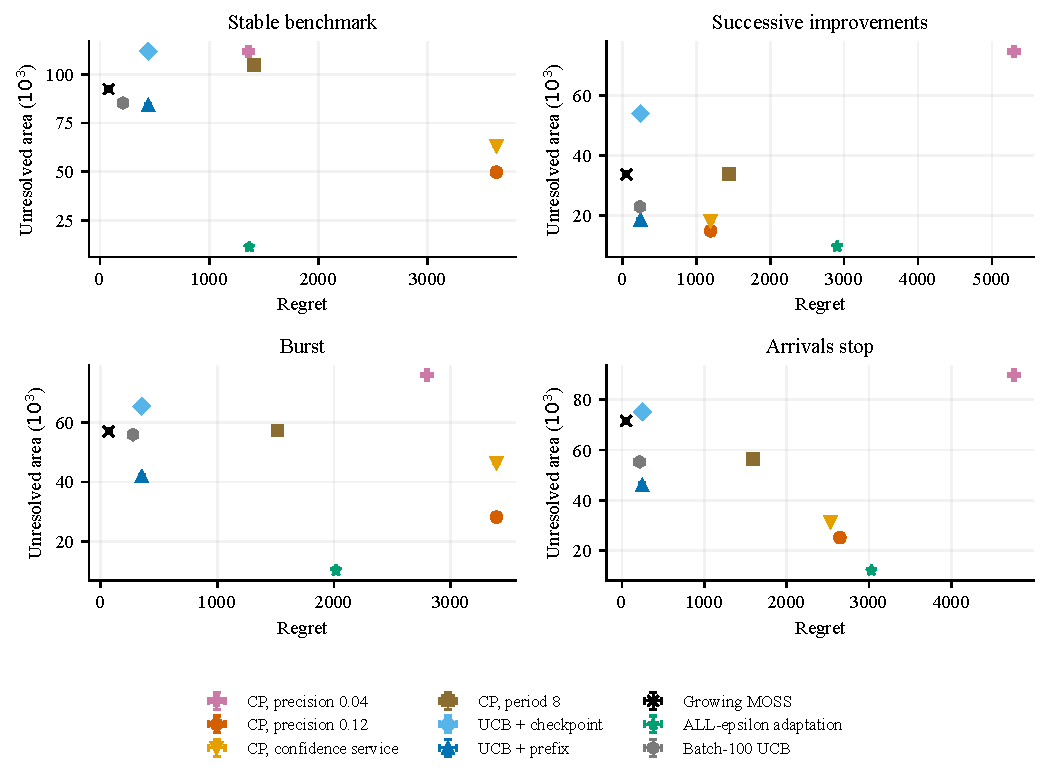
\includegraphics[width=.97\textwidth]{figures/fig_cost_area.pdf}
\caption{Regret and cumulative $\eta$-unresolved area for all nine methods.
Lower values on both axes are preferable. Error bars quantify Monte Carlo
uncertainty, not uncertainty in the theoretical reliability statement.
Neither checkpoint precision nor its allocation variants uniformly dominate
the confidence-based adaptation.}
\label{fig:cost-area}
\end{figure}

\subsubsection{What the comparisons show}

In all 640 finer-checkpoint runs, every available arm remains unresolved
at every time step. Five to eight arms are counted by the final
$\eta$-unresolved metric because that metric exempts the boundary band;
the remaining arms have not been classified. The resulting zero-error
record therefore does not establish useful classification at this budget.
Its charged unresolved area ranges from 74,820 to 111,784.
This is an observable limitation of the conservative construction, rather
than evidence that arrivals are intrinsically unmanageable at this budget.
The confidence-based adaptation resolves all $\eta$-separated arms by the
end in every replication of these four environments.

The coarser checkpoints reduce area substantially relative to UCB alone,
but can incur much larger regret. Under a stable benchmark, CP-FIFO has
mean regret 3629.9 and area 49,718, compared with 1367.8 and 11,306 for
ALL-$\varepsilon$ adaptation. The paired differences, CP-FIFO minus the
adaptation, are $2262.1$ (standard error $11.7$) for regret and $38{,}411.7$
(standard error $241.9$) for area. The adaptation also improves both
quantities in the burst environment. These comparisons do not support a
general numerical advantage of checkpoint FIFO over a strong
history-retaining identification rule.

In the successive-improvement environment, CP-FIFO instead occupies a
different cost point: regret 1194.7 and area 14,743, compared with 2905.8
and 9525 for the confidence-based adaptation. Here the paired regret
difference is $-1711.0$ (standard error $2.4$), while the area difference is
$5217.7$ (standard error $141.1$). These points do not isolate the benefit of task expiration. The adaptation
uses all 10,000 designated service pulls in this environment, while
coarse CP uses about 5,786; some remaining questions lie inside the
unpenalized boundary band. The lower regret may therefore partly reflect
a different stopping rule for reporting work. A comparison with the same
boundary tolerance and service requirement is needed to distinguish the
mechanisms. These observations do not estimate an optimal frontier.

Growing-MOSS has the smallest mean regret in all four environments,
between 52.0 and 77.3, while leaving substantially larger unresolved areas.
Low regret therefore provides little evidence of timely set maintenance.
Conversely, the explicit service rules pay for observations of inferior
arms. Reducing service from every second to every eighth pull generally
reduces regret and enlarges unresolved area. Replacing FIFO by the
confidence-driven checkpoint allocation does not uniformly improve either
criterion; allocation and the report's precision both matter.

\begin{figure}[t]
\centering
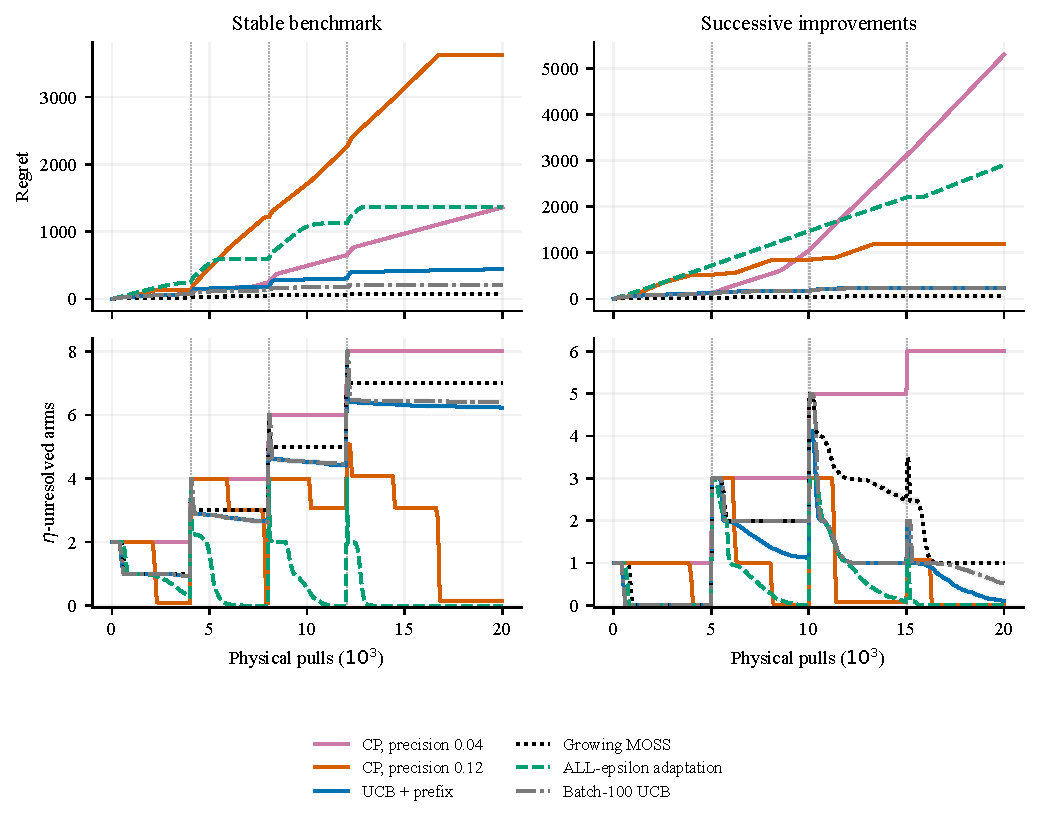
\includegraphics[width=.98\textwidth]{figures/fig_paths_pair1.pdf}
\caption{Mean regret and mean $\eta$-unresolved arm counts at the physical
sampling clock. Bands are 1.96 Monte Carlo standard errors; vertical dotted
lines mark arrivals. Stable and improving benchmarks are shown here;
the other environments appear in the supplement. The main six methods are
displayed; all nine methods and all sampled paths are retained in the released results.}
\label{fig:paths}
\end{figure}

For Batch100-UCB we additionally record the exact decomposition into
within-active regret, admission delay, and loss from previous reward
retirement. Its admission-delay contributions are $0$, $33.92$, $16.00$,
and $22.40$ in the four environments. No historical-retirement deficit
occurred in these runs. The largest discrepancy between total regret and
the sum of the three recorded components was below $3.1\times10^{-12}$.
The corresponding admission and retirement terms are identically zero for
the methods that admit every arm immediately and retain every arm for
reward selection. This accounting avoids attributing every loss outside
within-active learning to arrival delay.

There were no incorrect positive or negative reports in any of the 5760
runs. For one fixed environment and method, zero failures in 160
replications gives a one-sided 95\% upper confidence bound of 0.0186 on
its failure probability. This finite set of diagnostics does not establish
the uniform, all-environment reliability guarantee. Nor do these small
eight-arm experiments validate the asymptotic lower bounds, resolve the
critical logarithmic gap, or establish checkpoint optimality. They show
the practical cost of the conservative quotas and the importance of
comparing retained-history methods under both regret and maintenance
criteria.

\FloatBarrier
\section{Discussion}
\label{sec:discussion}

We studied stochastic multi-armed bandits with arriving arms, where the
available action set expands and performance is measured against the best
currently available arm. Arrival information discrepancy and a drifting
benchmark create repeated learning costs even though every arm has a
stationary reward law. The two-stage UCB-AA design addresses the information
imbalance by screening arrivals before full competition with incumbents.
The revised regret account separates learning, admission delay, and loss of
an earlier admitted benchmark. Its finite-budget guarantee is conditional
on the stated calibration and retains the admission-delay term explicitly.

The additional maintenance analysis makes precise a statistical question
that the original active-set comparison left open. A smaller internal set
does not establish reliable knowledge of the complete near-optimal set.
One uncertain arrival can obstruct many earlier certifications, and a
drifting benchmark can make difficult unresolved questions expire. The
broadcast and repeated-update results characterize costs arising from these
two effects. Their assumptions, including the restricted update family and
the different allowed area budgets, are part of the conclusions. The worst
area lower bound already occurs in a static initial batch; the temporary-task
results supply a separate dynamic mechanism.

UCB-AA and CP-UCB-AA serve different purposes in this analysis. The former
retains the original screening architecture. The latter is a constructive
reporting rule whose service precision is fixed in advance and whose
unconditional reward analysis does not require correct reports. Its
conservative checkpoints may be ineffective at moderate budgets, and its
numerical cost is not uniformly competitive. Neither a negative report
nor a smaller reported set is treated as a reduction in total storage.

The supplement supplies full proofs of the quantile lower bound in
Section~\ref{sec:tradeoff} and the compatible-window truncation result. It also gives eventual exact
classification by a separate revisable multiresolution construction when
arrivals stop, the final arm count is finite, and no arm lies on the
membership boundary. That conclusion does not apply to fixed-precision
checkpoints.

The general frontier under overlapping arrivals, automatic precision
selection, and a matching converse for deferred maintenance remain open.
The archived UCB-AA study also leaves a concrete empirical obligation:
the repaired procedure must be compared under the same admission and
retained-history rules before attributing a numerical gain to pre-elimination.
Contextual information, delayed feedback, and post-arrival reward drift
remain natural extensions of the original MAB-AA formulation.

\section*{Data and code availability}
No original empirical or human-subject outcome data were collected.
The original simulation configurations, endpoint records, source snapshots,
and figures are preserved separately from the new reporting experiments.
The release contains the 5,760 reporting runs, their fixed configuration,
code, and checks. The oncology illustration is the historical motivation
from the original submission, based on public approval records.

\bibliographystyle{plainnat}
\bibliography{references}
\end{document}
